\documentclass[10pt,a4paper]{article}
\usepackage[utf8]{inputenc}
\usepackage[T1]{fontenc}
\usepackage{amsmath}
\usepackage{amssymb}
\usepackage{hyperref}
\usepackage{graphicx}
\graphicspath{{./images/}}
\title{A Quick Dive into Ribosomes}
\author{R\^{i}mboi Eusebiu - grupa 332}

\begin{document}
	\maketitle
	
	\section{Introduction}
	The human cell is a complex organism that represents the fundamental part of any human body system or component. Being involved in so many areas and having so many functions, its internal mechanisms should be very powerful and clearly defined. For now, the one that is of interest for us in this short essay is the \textbf{protein synthesis}. But before diving in it, we must introduce the main actor in this process.
	
	The ribosome is a tiny cellular machine found close to the cell's nucleus, inside the cell, specialized in the creation of proteins. It's composed of 2 parts: ribosomal RNA (rRNA) and various proteins. The process by which these micro-organisms get created is called \textbf{Ribosome Biogenesis} and implies involvement of more than two hundred proteins, mRNA and a lot of energy. Since ribosomes' only role is in proteins synthesis, this gives us a hint on why this process is so crucial to each one of us.
	
	As a side fact, ribosomes were initially named \textbf{Palade granules} after the Romanian doctor and biologist that firstly investigated them \textbf{George Emil Palade}.
	
	\begin{figure}[h]
		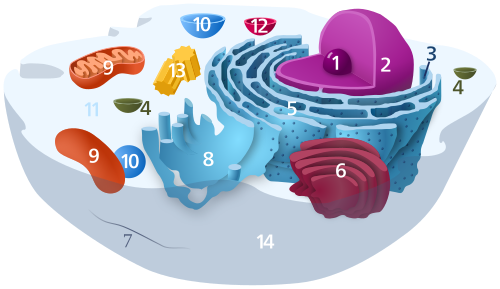
\includegraphics[width=0.7 \textwidth]{cell.png}
		\caption{Inside a cell: 1. Nucleolus; 2. Nucleus; 3. Ribosome (dots as part of 5); 4. Vesicle; 5. Rough endoplasmic reticulum; 6. Golgi apparatus (or, Golgi body); 7. Cytoskeleton; 8. Smooth endoplasmic;  reticulum; 9. Mitochondrion; 10. Vacuole; 11. Cytosol (fluid that contains organelles; with which, comprises cytoplasm); 12. Lysosome; 13. Centrosome; 14. Cell membrane}
		\href{https://en.wikipedia.org/wiki/Ribosome}{Source: https://en.wikipedia.org/wiki/Ribosome}
	\end{figure}
	
	\section{Proteins Synthesis}
	When it comes to living organisms, there is no doubt that their existence depends on the proteins: even though cells require glucose as fuel, for their functions (communication, genes activation, fuel processing, physical properties, even ribosomes creation) proteins are the ones making that possible. Thus, this raises the question of how these little and crucial chemicals are born. Having that in place, let's explore now how the magic is done.
	
	Firstly, there are the RNA polymerase enzymes which are responsible for binding to the DNA and copying the portions of it which are activated by the \textbf{transformation factor (TF)} proteins (they dictate what type of cell is that), into new components called RNA. This operation is crucial to maintain the integrity of DNA - every mutation takes place on the RNA, which is a prone to mutations version of the DNA, mostly because of its single stranded structure; otherwise the DNA could risk of being changed that could lead to potentially severe problems.
	
	After that, by the time the RNA structures are formed, they are sent outside the nucleus in the form of mRNA. Then the ribosome enters the scene: it firstly binds to this freely roaming mRNA and reads the first 3 nucleotides (codons) from the sequence. After that, by random thermal motions (called diffusions), the high number of tRNA molecules present in the cytoplasm try to match the pattern of that processed mRNA inside the ribosome: if they don't match, the tRNA leaves, else a new amino-acid is added. Now, since the tRNA is already bound to the amino-acid described by its 3 nucleotides in the moment they are in cytoplasm, when a match occurs between the 2 sets of codons, the amino-acid transported by the tRNA is released and connected to the chain of amino-acids previously formed. This event triggers the removal of now empty tRNA and processing of the next 3 nucleotides from the bound mRNA. This process repeats until any of the \textbf{UAG}, \textbf{UGA} or \textbf{UAA} is met; as a side note, every mRNA molecule includes the \textbf{AUG} codon at the beginning, to mark the start of the chain.
	
	It's worth mentioning that there are only 20 $\alpha$ amino-acids the cell can generate, so that means that from the total of $64$ nucleotides combinations, different sequences can lead to the same amino-acid, or may indicate the beginning or termination of the chain as presented above.
	
	In the end, after the termination codon, the chain of amino-acids that now forms a polypeptide and by folding it we get a third-dimension protein.
	
	\begin{figure}[h]
		\centering
		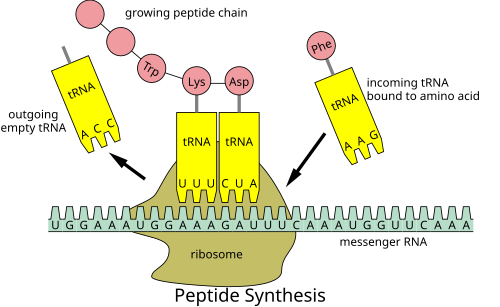
\includegraphics[width=0.4\textwidth]{peptides_formation.png}
		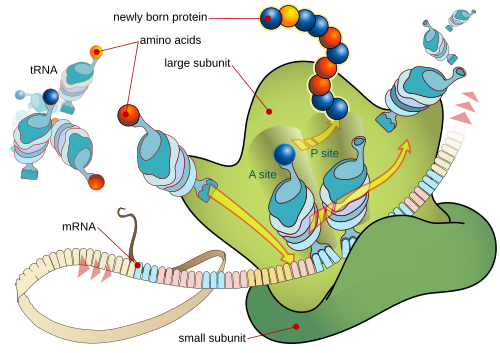
\includegraphics[width=0.4\textwidth]{mRNA_translation.png}
		\caption{Proteins Synthesis in Action}
		\href{https://en.wikipedia.org/wiki/Ribosome}{Source: https://en.wikipedia.org/wiki/Ribosome}
	\end{figure}
	
	\section*{Bibliography}
	\begin{description}
		\item [$\bullet$ \href{https://en.wikipedia.org/wiki/Ribosome}{Wikipedia}]
		\item [$\bullet$ \href{https://www.youtube.com/watch?v=O2Nu_Lo1FGo}{YouTube}]
	\end{description}

\end{document}

